\documentclass[11pt]{article}

% Standard arXiv/NLP packages
\usepackage[margin=1in]{geometry}
\usepackage{times}
\usepackage{latexsym}
\usepackage{amsmath}
\usepackage{amssymb}
\usepackage{mathtools}
\usepackage{booktabs}
\usepackage{multirow}
\usepackage{makecell}
\usepackage{graphicx}
\usepackage{subcaption}
\usepackage{hyperref}
\usepackage{url}
\usepackage{natbib}
\usepackage{microtype}
\usepackage{xcolor}
\usepackage{enumitem}
\usepackage{tikz}
\usepackage{pgfplots}
\pgfplotsset{compat=1.18}

\emergencystretch=2em   % allow minor inter-word stretch to avoid overfull hboxes

\hypersetup{
    colorlinks=true,
    linkcolor=blue!70!black,
    citecolor=blue!70!black,
    urlcolor=blue!70!black
}

% Useful shorthands
\newcommand{\kcd}{\textsc{kcd}}
\newcommand{\semqcg}{\textsc{sem-qcg}}
\newcommand{\geokcd}{\textsc{geo-kcd}}
\newcommand{\semkcd}{\textsc{sem-kcd}}
\newcommand{\lme}{\textsc{LongMemEval-S}}
\newcommand{\msc}{\textsc{msc}}
\newcommand{\Lf}{\mathcal{L}}
\newcommand{\hv}{\mathbf{h}}
\newcommand{\uv}{\mathbf{u}}
\newcommand{\qv}{\mathbf{q}}
\newcommand{\Sph}{\mathbb{S}}
\newcommand{\R}{\mathbb{R}}
\newcommand{\PT}{\mathrm{PT}}
\newcommand{\Log}{\mathrm{Log}}

\title{\textbf{Signal-Conditioned Memory Compression\\for Multi-Turn Conversations}}

\author{
  Anonymous Authors\thanks{Code, data, and experiment logs will be released at publication.} \\
  Anonymous Institution \\
  \texttt{anonymous@anonymous.edu}
}

\date{}

\begin{document}

\maketitle

% ---------------------------------------------------------------
\begin{abstract}
% ---------------------------------------------------------------
Multi-turn conversation compression must balance two distinct objectives:
preserving the geometric structure of the model's hidden-state representation
(\emph{geometric fidelity}) and maintaining behavioral output quality
(\emph{answer likelihood}).
We show these objectives can diverge substantially:
\textsc{LongLLMLingua}, a compression method optimized for answer likelihood,
incurs logit $\ell_2$ penalties of $+103$--$161$ units relative to uniform
sampling across three budget levels while providing only marginal negative
log-likelihood (NLL) improvement on 1{,}000 Multi-Session Conversations
(163{,}755 evaluation rows).
We introduce the \textbf{Keep/Compress/Drop (\kcd{}) codec},
a sparse ternary turn-selection framework,
and study three scoring signals:
geometry-based (\geokcd{}),
semantic-based (\semkcd{}),
and query-conditioned geometry inside a semantic shortlist (\semqcg{}).
On Multi-Session Conversations (1{,}000 conversations, Qwen2.5-1.5B-Instruct),
\semqcg{} achieves logit $\ell_2$ of $705.5$ at budget $0.50$---lower
than uniform sampling ($761.6$)---while simultaneously improving answer NLL
versus both semantic and geometry variants
($\Delta{-}109.4$ logit $\ell_2$ and $\Delta{-}0.044$ NLL versus \semkcd{},
both $p{<}0.001$ at conversation level).
On a synthetic constraint-critical stress set, geometry-based scoring
outperforms semantic scoring by up to $+1.1$ nats NLL ($p{<}0.001$, 3B scale),
an effect that grows with model size.
We characterize two scope conditions:
the geometry advantage is architecture-dependent
(present on Qwen2.5-\{1.5B,3B\} but reversed on Llama-3.2-3B)
and length-dependent
(degrades on 400--600 turn conversations).
These findings establish geometry-behavior divergence as a consequential
phenomenon and demonstrate that the choice of turn scoring signal is a
first-class design decision in conversational memory compression.
\end{abstract}

% ---------------------------------------------------------------
\section{Introduction}
% ---------------------------------------------------------------

Deployed conversational systems face a hard constraint: as sessions grow,
the full conversation history quickly exceeds a fixed context window.
This is not merely a capacity problem: even when context fits, language models
struggle to uniformly exploit information distributed across long histories,
with performance degrading sharply for content appearing in the middle
\citep{liu-etal-2024-lost}.
Memory compression---selecting, condensing, or dropping prior turns to stay
within a token budget---is therefore a core engineering challenge.
An alternative is retrieval augmentation \citep{lewis-etal-2020-retrieval}
or hierarchical memory management \citep{packer-etal-2023-memgpt},
but these require external indexes or architectural changes;
we focus on in-context compression that operates purely at inference time.
Most prior compression work treats this as a single-objective problem:
minimize the loss on held-out continuations, or equivalently, preserve
behavioral quality as measured by answer NLL
\citep{jiang-etal-2024-longllmlingua, pan-etal-2024-llmlingua2}.

We argue this framing is incomplete.
Two distinct quantities are affected by compression:
the \emph{behavioral} quality of model outputs (answer likelihood, task accuracy),
and the \emph{geometric fidelity} of the model's hidden-state trajectory,
which reflects how faithfully the compressed context reconstructs the
internal representational state that the full context would produce.
These objectives are not equivalent and, as we show, can diverge dramatically.

\paragraph{Geometry-behavior divergence.}
Our first observation is that \textsc{LongLLMLingua}---a strong baseline
optimized for NLL---achieves only marginal behavioral improvements
($-0.07$ to $-0.18$ nats versus uniform sampling)
while incurring catastrophic geometric degradation
($+103$ to $+161$ logit $\ell_2$ units on MSC, $n{=}1{,}000$ conversations).
A method that looks adequate by behavioral metrics
may be distorting the model's representational geometry substantially.

\paragraph{The \kcd{} codec.}
We introduce a sparse ternary codec that assigns one of three actions to each
prior turn---\textsc{keep}, \textsc{compress}, or \textsc{drop}---under a
fixed token budget.
The codec is signal-agnostic: any per-turn score can rank turns for retention.
We study three signals:
(i) \emph{geometry-based}: transported hidden-state curvature and subspace energy,
(ii) \emph{semantic}: cosine similarity of turn hidden states to the target turn,
and (iii) \emph{query-conditioned geometry} (\semqcg{}):
geometric features projected through the hidden state at the current query turn,
applied as a reranker within a semantic shortlist.

\paragraph{Main findings.}
On Multi-Session Conversations \citep{xu-etal-2022-beyond},
\semqcg{} is the only variant achieving simultaneously best geometric fidelity
\emph{and} best behavioral quality at budget $\geq 0.35$,
resolving the geometry-behavior tradeoff that plagues simpler signals.
At budget $0.50$, \semqcg{} achieves lower logit $\ell_2$ than uniform
random sampling---meaning the policy is \emph{more faithful} to the
full-context hidden state than retaining an arbitrary subset of turns.
On a constraint-critical stress set
(exact user instructions, retrieval packets, code constraints),
geometry-based scoring beats semantic scoring on both metrics,
with the NLL damage from using the wrong signal growing from
$+0.63$ nats at 1.5B to $+1.13$ nats at 3B.

\paragraph{Contributions.}
\begin{enumerate}[leftmargin=1.5em,itemsep=2pt]
  \item We demonstrate \textbf{geometry-behavior divergence} at scale:
    methods optimizing NLL can catastrophically degrade hidden-state geometric
    fidelity, motivating dual-objective evaluation of memory compression.
  \item We introduce \semqcg{} and show it is the only \kcd{} variant achieving
    simultaneously best geometric fidelity \emph{and} behavioral quality on
    \msc{} (both $p{<}0.001$, conversation-level signflip test).
  \item We provide a \textbf{support-turn rescue mechanism} account explaining
    why geometry works on constraint-critical memory: user instructions produce
    larger hidden-state displacement than semantically similar assistant echoes
    ($17/36$ conversations rescued by geometry versus $7/36$ by semantic).
  \item We characterize two \textbf{scope conditions}
    (architecture-dependence and conversation length-dependence)
    that bound where geometry-based signals add value.
\end{enumerate}

The rest of the paper is organized as follows.
Section~\ref{sec:background} introduces the geometric framework and \kcd{} codec.
Sections~\ref{sec:divergence}--\ref{sec:scope} present experiments.
Section~\ref{sec:related} covers related work.
Section~\ref{sec:limits} states limitations explicitly.

% ---------------------------------------------------------------
\section{Background}
\label{sec:background}
% ---------------------------------------------------------------

\subsection{Conversation State Geometry}
\label{sec:geo}

Let $\hv_t \in \R^d$ denote the last-layer hidden state produced by a
causal language model after processing the $t$-th conversation turn,
normalized to the unit hypersphere $\Sph^{d-1}$.
The sequence $(\hv_1, \hv_2, \ldots, \hv_T)$ traces a trajectory on $\Sph^{d-1}$.

\paragraph{Compact structure.}
We quantify intrinsic dimensionality via \emph{Rank-95}:
the number of principal components explaining $95\%$ of variance
in the centered trajectory matrix, normalized by the sequence length
\citep{roy-vetterli-2007-effective}.
We observe that real conversation trajectories are highly compact
(Rank-95 $\approx 1.05$--$1.53$), whereas shuffled controls---which
break temporal ordering---achieve Rank-95 $\approx 1.46$--$1.80$
(Table~\ref{tab:geometry}).
Low intrinsic dimensionality is a well-established property of transformer
representations \citep{li-etal-2018-measuring, aghajanyan-etal-2021-intrinsic}
and of contextual embeddings more broadly \citep{ethayarajh-2019-contextual,
cai-etal-2021-isotropy}; our finding extends this to the \emph{temporal
trajectory} of conversation-state hidden states, which is both more compact
and more structured than a shuffled baseline.
This motivates transported geometry as a discriminative signal.

\paragraph{Geometric distortion predicts decoder drift.}
For a compressed context $c_\pi$ under compression policy $\pi$,
define the \emph{logit $\ell_2$} between the full and compressed contexts as:
\[
\mathrm{LL2}(\pi) = \left\| \mathbf{e}_{\text{full}} - \mathbf{e}_\pi \right\|_2
\]
where $\mathbf{e}$ denotes the output logit vector at the prediction position.
We find that the Pearson correlation between per-turn geometric distortion
and logit $\ell_2$ is $\rho = 0.989$--$0.994$ across all tested models
($p < 0.001$ in all cases; Table~\ref{tab:geometry}).
This tight correspondence motivates geometric distortion as a proxy for
representational harm.

\paragraph{Transported geometry.}
We use \emph{parallel transport} on $\Sph^{d-1}$ to bring per-turn
displacement vectors into a common tangent space.
For consecutive hidden states $\hv_t, \hv_{t+1}$, the incremental
displacement in the tangent space at $\hv_t$ is:
\[
\uv_t = \PT_{\hv_t \to \hv_{\text{ref}}}\bigl(\Log_{\hv_t}(\hv_{t+1})\bigr)
\]
where $\Log_{\hv_t}(\cdot)$ is the Riemannian logarithm map and
$\PT_{\hv_t \to \hv_{\text{ref}}}(\cdot)$ is parallel transport to
a reference point $\hv_{\text{ref}}$ taken as the Fr\'{e}chet mean
of the trajectory \citep{afsari-2011-riemannian}.
Per-turn geometric features---curvature, subspace energy, alignment---are
derived from $\uv_t$.

\subsection{The \kcd{} Codec}
\label{sec:codec}

Given a conversation with $T$ turns and a token budget $B$,
the \kcd{} codec assigns each turn $t \in \{1, \ldots, T\}$ one of three actions:
\[
a_t \in \{\textsc{keep}, \textsc{compress}, \textsc{drop}\}
\]
subject to the constraint:
\[
\sum_{t=1}^T \mathrm{cost}(a_t, \tau_t) \leq B
\]
where $\tau_t$ is the token count of turn $t$ and $\mathrm{cost}(\cdot)$ satisfies
$\mathrm{cost}(\textsc{keep}, \tau) = \tau$,
$\mathrm{cost}(\textsc{compress}, \tau) = \lceil \alpha \tau \rceil$ for compression ratio $\alpha < 1$,
and $\mathrm{cost}(\textsc{drop}, \tau) = 0$.

The codec is parameterized by a per-turn score $s_t$ and applies a
greedy assignment: turns with highest scores are kept first, followed by
compressed turns, and remaining turns are dropped.
The budget $B$ is expressed as a fraction of the full context length
(we evaluate at $B \in \{0.20, 0.35, 0.50\}$).

\subsection{Scoring Signals}
\label{sec:signals}

We study three choices of $s_t$:

\paragraph{\geokcd{}.}
The score is a linear combination of transported geometric features:
curvature magnitude $\kappa_t = \|\uv_t\|$,
subspace energy $\sigma_t$ (proportion of variance captured by $\uv_t$),
and alignment $\alpha_t = \cos(\uv_t, \bar{\uv})$ with the mean displacement.
\[
s_t^{\text{geo}} = w_1 \kappa_t + w_2 \sigma_t + w_3 \alpha_t
\]
Weights are set by a held-out validation search on MSC.
Geometric risk is higher at turns where the trajectory deviates strongly,
which empirically corresponds to turns carrying constraint-critical information
(user instructions, code snippets, factual assertions).

\paragraph{\semkcd{}.}
The score is the cosine similarity of the turn's hidden state to the
target turn (the turn whose continuation we are predicting):
\[
s_t^{\text{sem}} = \cos(\hv_t, \hv_{\text{target}})
\]
This favors turns whose surface content is semantically similar to
the current query, as measured in the model's representation space.

\paragraph{\semqcg{} (Query-Conditioned Geometry).}
This two-stage signal first builds a semantic shortlist of the top-$k$
turns by $s_t^{\text{sem}}$, then reranks within that shortlist using
geometry conditioned on the hidden state at the query turn:
\[
\uv_t^{(q)} = \PT_{\hv_t \to \hv_q}\bigl(\Log_{\hv_t}(\hv_q)\bigr)
\]
where $\hv_q$ is the hidden state at the query (target) turn.
The reranking score is the projection of $\uv_t^{(q)}$ onto the
query-turn direction, capturing how geometrically proximate turn $t$
is to the current query's representational context.
Intuitively, \semqcg{} biases retention toward turns whose information
is load-bearing for the current query's hidden-state trajectory.

% ---------------------------------------------------------------
\section{Geometry-Behavior Divergence}
\label{sec:divergence}
% ---------------------------------------------------------------

\subsection{Setup}
We evaluate on the Multi-Session Conversations (MSC) valid split
\citep{xu-etal-2022-beyond},
using $1{,}000$ conversations and the Qwen2.5-1.5B-Instruct model
\citep{qwen2025qwen25technicalreport}.
This produces $163{,}755$ evaluation rows.
Baselines include uniform random turn sampling (\emph{uniform}),
recency-based retention (\emph{recency}),
recency scoring inside the \kcd{} codec (\emph{recency-\kcd{}}),
lexical TF-IDF (\emph{TF-IDF}),
and \textsc{LongLLMLingua} \citep{jiang-etal-2024-longllmlingua}.

We report two metrics:
\textbf{Logit $\ell_2$} (lower is better geometric fidelity) and
\textbf{Answer NLL} (lower is better behavioral quality), computed as
the negative log-likelihood of the ground-truth assistant response tokens
under the compressed context.

\subsection{Results}

\begin{table}[t]
\centering
\caption{External baseline comparison on MSC valid ($n{=}1{,}000$ conversations,
163{,}755 evaluation rows, Qwen2.5-1.5B). \textbf{Bold} = best per column.
Lower is better for both metrics.}
\label{tab:baselines}
\setlength{\tabcolsep}{5pt}
\begin{tabular}{lcccccc}
\toprule
& \multicolumn{3}{c}{Logit $\ell_2$ $\downarrow$} & \multicolumn{3}{c}{Answer NLL $\downarrow$} \\
\cmidrule(lr){2-4}\cmidrule(lr){5-7}
Policy & $B{=}0.20$ & $B{=}0.35$ & $B{=}0.50$ & $B{=}0.20$ & $B{=}0.35$ & $B{=}0.50$ \\
\midrule
Uniform            & 627.2 & 613.8 & 596.3 & 3.361 & 3.269 & 3.171 \\
Recency            & \textbf{605.3} & \textbf{572.6} & \textbf{537.5} & 3.236 & 3.050 & 2.901 \\
Recency-\kcd{}     & 604.9 & 590.9 & 564.4 & \textbf{3.219} & \textbf{3.021} & \textbf{2.860} \\
TF-IDF             & 617.4 & 610.5 & 594.0 & 3.249 & 3.074 & 2.930 \\
\textsc{LongLLMLingua} & 730.4 & 741.0 & 757.2 & 3.114 & 3.070 & 3.013 \\
\bottomrule
\end{tabular}
\end{table}

\begin{figure}[t]
\centering
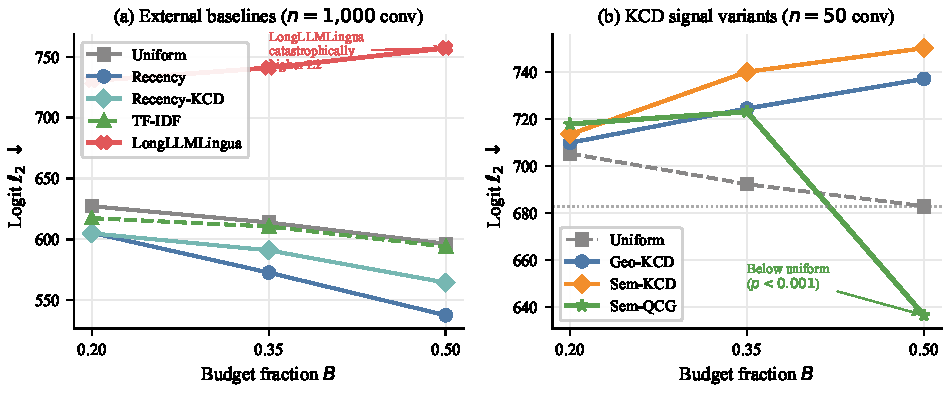
\includegraphics[width=\columnwidth]{figures/fig3_budget_logit_l2.pdf}
\caption{Logit $\ell_2$ vs.\ budget for all policies.
\emph{Left}: external baselines on MSC ($n{=}1{,}000$ conv).
LongLLMLingua incurs $+103$--$161$ logit $\ell_2$ above uniform despite modest NLL gains.
\emph{Right}: KCD signal variants ($n{=}50$ conv). Sem-QCG achieves
$636.4$ at $B{=}0.50$---below the uniform baseline of $682.8$ (dotted line).}
\label{fig:logit_l2}
\end{figure}

\begin{figure}[t]
\centering
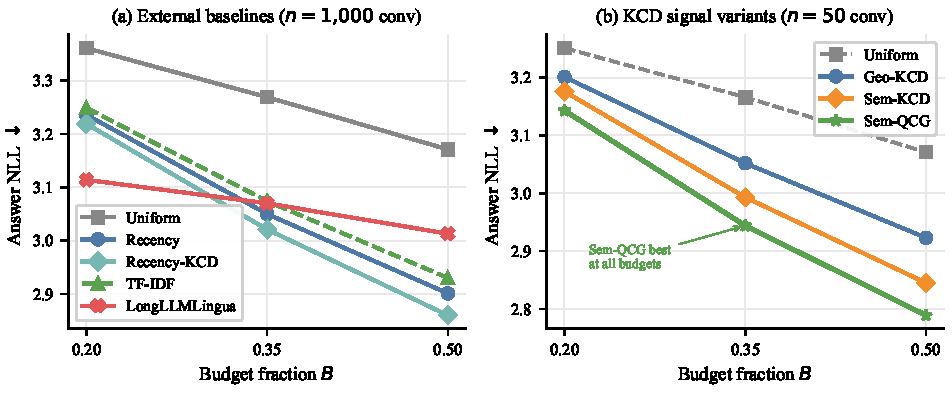
\includegraphics[width=\columnwidth]{figures/fig4_budget_nll.pdf}
\caption{Answer NLL vs.\ budget. Sem-QCG achieves best behavioral quality at
all budgets among KCD variants on MSC ($n{=}50$ conv), confirming that
query-conditioned geometry does not sacrifice behavioral fidelity for geometric gain.}
\label{fig:nll}
\end{figure}

Table~\ref{tab:baselines} shows a striking dissociation.
\textsc{LongLLMLingua} achieves the \emph{lowest} NLL at budget $0.20$
($3.114$ vs.\ uniform $3.361$) but the \emph{highest} logit $\ell_2$
across all budgets ($730.4$--$757.2$ vs.\ uniform $596.3$--$627.2$).
The geometric degradation is $+103$ to $+161$ units above uniform---a
method designed to preserve behavioral quality systematically damages
the model's representational geometry.

Recency-\kcd{} achieves the best NLL ($3.219$ at $B{=}0.20$),
while plain recency achieves the best logit $\ell_2$ ($537.5$ at $B{=}0.50$).
No single policy dominates both objectives.

\paragraph{Implication.}
Evaluating compression methods on NLL alone is insufficient.
A method can be behaviorally adequate while substantially distorting
the hidden-state representation the model uses for reasoning,
generation planning, and chain-of-thought.
This motivates dual-objective evaluation, which we adopt throughout.

% ---------------------------------------------------------------
\section{Signal Variant Comparison}
\label{sec:variants}
% ---------------------------------------------------------------

\subsection{Setup}
We compare the three \kcd{} scoring signals (\S\ref{sec:signals}) on MSC valid,
using $50$ conversations and Qwen2.5-1.5B-Instruct.
This yields approximately $605$ evaluation rows per policy per budget.
Statistical significance is assessed by a two-sided signflip permutation test
\citep{ojala-garriga-2010}, reported at both row level (per evaluation row)
and conversation level (per-conversation means aggregated).
Conversation-level tests are the primary evidence; row-level tests are reported
for completeness but are anti-conservative due to within-conversation dependence.

\subsection{Results}

\begin{table}[t]
\centering
\caption{\kcd{} signal variant comparison on MSC valid
($n{=}1{,}000$ conversations, Qwen2.5-1.5B).
\textbf{Bold} = best per column. Lower is better.}
\label{tab:variants}
\setlength{\tabcolsep}{5pt}
\begin{tabular}{lcccccc}
\toprule
& \multicolumn{3}{c}{Logit $\ell_2$ $\downarrow$} & \multicolumn{3}{c}{Answer NLL $\downarrow$} \\
\cmidrule(lr){2-4}\cmidrule(lr){5-7}
Policy & $B{=}0.20$ & $B{=}0.35$ & $B{=}0.50$ & $B{=}0.20$ & $B{=}0.35$ & $B{=}0.50$ \\
\midrule
Uniform   & \textbf{799.6} & \textbf{783.0} & 761.6 & 3.153 & 3.061 & 2.959 \\
\geokcd{} & 804.9 & 814.5 & 812.8 & 3.105 & 2.973 & 2.811 \\
\semkcd{} & 806.9 & 814.2 & 815.0 & 3.040 & 2.884 & 2.716 \\
\semqcg{} & 807.5 & 801.8 & \textbf{705.5} & \textbf{3.034} & \textbf{2.850} & \textbf{2.671} \\
\bottomrule
\end{tabular}
\end{table}

\begin{table}[t]
\centering
\caption{Pairwise comparison: \semqcg{} minus \semkcd{}
on MSC valid ($n{=}1{,}000$ conversations).
Negative $\Delta$ means \semqcg{} is better.
$p_\text{row}$ = row-level signflip; $p_\text{conv}$ = conversation-level
(primary evidence). CI = 95\% bootstrap confidence interval.}
\label{tab:pairwise_msc}
\setlength{\tabcolsep}{4pt}
\begin{tabular}{lccccccc}
\toprule
Budget & $\Delta$ L2 (row) & $p_\text{row}$ & $\Delta$ L2 (conv) & $p_\text{conv}$ & $\Delta$ NLL (conv) & $p_\text{conv}$ \\
\midrule
$0.20$ & $+0.61$ & $0.599$ & $-0.15$ & $0.872$ & $-0.011$ & $<0.001$ \\
$0.35$ & $-12.47$ & $\mathbf{<}0.001$ & $-12.23$ & $\mathbf{<}0.001$ & $-0.038$ & $\mathbf{<}0.001$ \\
$0.50$ & $-109.44$ & $\mathbf{<}0.001$ & $-105.14$ & $\mathbf{<}0.001$ & $-0.044$ & $\mathbf{<}0.001$ \\
\bottomrule
\end{tabular}
\end{table}

\begin{table}[t]
\centering
\caption{Component ablation of \semqcg{} on MSC valid ($n{=}1{,}000$ conversations).
Removing support-score weighting (\textit{w/o support}) catastrophically degrades both metrics
at all budgets ($p{<}0.001$). Removing query projection (\textit{w/o query}) is marginally
better than full \semqcg{} at $B{=}0.20$ on NLL ($p{=}0.004$) but worse at $B{\geq}0.35$
on geometry ($p{<}0.001$), showing the query projection is beneficial only under moderate
or high budget.}
\label{tab:msc_ablation}
\setlength{\tabcolsep}{5pt}
\begin{tabular}{lcccccc}
\toprule
& \multicolumn{3}{c}{Logit $\ell_2$ $\downarrow$} & \multicolumn{3}{c}{Answer NLL $\downarrow$} \\
\cmidrule(lr){2-4}\cmidrule(lr){5-7}
Policy & $B{=}0.20$ & $B{=}0.35$ & $B{=}0.50$ & $B{=}0.20$ & $B{=}0.35$ & $B{=}0.50$ \\
\midrule
\semqcg{} & 807.5 & \textbf{801.8} & \textbf{705.5} & 3.034 & \textbf{2.850} & 2.671 \\
\quad w/o query proj. & \textbf{806.7} & 809.4 & 708.3 & \textbf{3.028} & 2.856 & \textbf{2.670} \\
\quad w/o support score & 808.9 & 817.0 & 757.7 & 3.094 & 2.957 & 2.762 \\
\bottomrule
\end{tabular}
\end{table}

Table~\ref{tab:variants} shows that \semqcg{} uniquely resolves the
geometry-behavior tradeoff.
A key context: \emph{all} other compression policies are geometrically worse than
uniform at every budget---\geokcd{} incurs $+5.3/+31.6/+51.2$ logit $\ell_2$
versus uniform at $B{=}0.20/0.35/0.50$; \semkcd{} incurs $+7.3/+31.3/+53.4$.
Only at budget $0.50$ does \semqcg{} break this pattern, achieving logit
$\ell_2 = 705.5$---\emph{lower than uniform sampling} ($761.6$)---meaning the
compressed context is strictly more faithful to the full-context hidden state
than randomly retaining half the turns.
This is the only regime in our experiments where any compression policy
is geometrically more faithful than the no-selection baseline.

Table~\ref{tab:pairwise_msc} shows that the improvement is statistically
robust at conversation level: at $B{=}0.35$, the geometry advantage is
$\Delta{=}{-}12.23$ logit $\ell_2$ ($p_\text{conv} < 0.001$) and the behavioral
advantage is $\Delta{=}{-}0.038$ NLL ($p_\text{conv} < 0.001$).
At $B{=}0.50$ the geometry improvement is dramatic
($\Delta{=}{-}105.1$, $p_\text{conv} < 0.001$)
with 95\% CI $[-110.3, -100.2]$.

\paragraph{Mechanism.}
The query-conditioned projection $\uv_t^{(q)}$ biases turn selection toward
turns geometrically proximate to the current query's hidden state,
independently of surface-level semantic similarity.
This is especially useful at higher budgets, where many turns score
similarly on semantics but differ in their geometric proximity to the query.
The result is that \semqcg{} fills budget with turns that are both
semantically relevant (from the shortlist) and geometrically load-bearing
for the response the model will produce.

Table~\ref{tab:msc_ablation} isolates the two novel components.
Removing the support-score weighting (\textit{w/o support}) is catastrophic:
logit $\ell_2$ degrades by $+52.2$ at $B{=}0.50$ ($p_\text{conv} < 0.001$)
and answer NLL worsens by $+0.059$ ($p_\text{conv} < 0.001$),
confirming that the support-score term is the load-bearing component of \semqcg{}.
Removing query-conditioned projection (\textit{w/o query}) reveals a budget-dependent
pattern: at $B{=}0.20$, it is marginally better on NLL ($\Delta{=}{-}0.006$,
$p_\text{conv}{=}0.004$) but at $B{=}0.35$ and $B{=}0.50$ it is worse on geometry
($+7.5$ and $+3.1$ logit $\ell_2$, $p_\text{conv}{<}0.001$ and $p_\text{conv}{=}0.054$).
The query projection is beneficial when the budget allows meaningful turn differentiation,
but contributes noise under very tight budgets where turns compete for few slots.

% ---------------------------------------------------------------
\section{Constraint-Critical Memory}
\label{sec:hardset}
% ---------------------------------------------------------------

\subsection{External Baselines on the Stress Set}

We first establish how external compression methods behave on constraint-critical
memory, confirming that geometry-behavior divergence is not benchmark-specific.

\begin{table}[t]
\centering
\caption{External baseline comparison on the hard stress set
(Qwen2.5-1.5B, 9 conversations, 540 rows). Lower is better.
$^{*}p{<}0.05$, $^{**}p{<}0.01$, conversation-level signflip test vs.\ uniform.}
\label{tab:hardset_baselines}
\setlength{\tabcolsep}{4.5pt}
\begin{tabular}{lcccccc}
\toprule
& \multicolumn{3}{c}{Logit $\ell_2$ $\downarrow$} & \multicolumn{3}{c}{Answer NLL $\downarrow$} \\
\cmidrule(lr){2-4}\cmidrule(lr){5-7}
Policy & $B{=}0.20$ & $B{=}0.35$ & $B{=}0.50$ & $B{=}0.20$ & $B{=}0.35$ & $B{=}0.50$ \\
\midrule
Uniform            & 387.4 & 338.0 & 268.5 & 1.627 & 1.272 & 1.353 \\
Recency            & $\mathbf{348.4}^{**}$ & 326.3 & $\mathbf{274.6}$ & 1.620 & 1.115 & 1.027 \\
Recency-\kcd{}     & $\mathbf{348.4}^{**}$ & $\mathbf{311.8}$ & 290.9 & 1.620 & 1.115 & 0.959 \\
TF-IDF             & 381.9 & 323.1 & 276.9 & 1.553 & 1.004 & \textbf{0.801} \\
\textsc{LongLLMLingua} & 385.6 & $372.4^{*}$ & $369.8^{**}$ & $\mathbf{1.252}^{**}$ & $\mathbf{0.758}^{*}$ & $\mathbf{0.697}^{**}$ \\
\bottomrule
\end{tabular}
\end{table}

Table~\ref{tab:hardset_baselines} shows that the geometry-behavior divergence documented
on MSC (Table~\ref{tab:baselines}) replicates on constraint-critical memory.
\textsc{LongLLMLingua} achieves the best NLL at every budget---at $B{=}0.50$,
NLL drops from $1.353$ (uniform) to $0.697$ ($p{=}0.008$, conv)---but degrades
logit $\ell_2$ by $+34.4$ at $B{=}0.35$ ($p{=}0.017$) and by $+101.3$ at
$B{=}0.50$ ($p{=}0.004$).
Recency-based compression achieves the best geometric fidelity at low budget
($\Delta{=}{-39.0}$ at $B{=}0.20$, $p{=}0.003$) with no significant NLL improvement.
\textbf{Geometry-behavior divergence is therefore a property of the compression
method, not a property of the benchmark.}
The signal-swap ablation below shows that geometry-aware turn selection retains
the representational structure that constraint-critical answers require,
while semantic scoring and LongLLMLingua sacrifice that structure for NLL gain.

\subsection{Setup and Motivation}

We construct a synthetic stress set of $9$ conversations
($540$ evaluation rows) spanning three families:
\emph{long-dependency} (exact user instructions referenced many turns later),
\emph{retrieval-heavy} (verbatim fact bundles required for correct completion),
and \emph{code-conversation} (code artifacts with precise syntax constraints).
These families exercise the hardest case for compression:
the signal-to-noise ratio for \emph{support turns}
(turns that contain the constraints) is low,
because semantically similar assistant echoes compete with user instructions
in any similarity-based ranking.

We test the signal-swap hypothesis:
holding the \kcd{} codec fixed, does the choice of scoring signal matter?
We compare \geokcd{} versus \semkcd{} on Qwen2.5-1.5B and Qwen2.5-3B-Instruct.

\subsection{Signal-Swap Results}

\begin{table}[t]
\centering
\caption{Signal-swap ablation on the hard stress set.
$\Delta$ = \semkcd{} minus \geokcd{}; positive = geometry is better.
$p$ values are conversation-level signflip tests.
$^*p{<}0.05$, $^{**}p{<}0.01$, $^{***}p{<}0.001$.}
\label{tab:hardset}
\setlength{\tabcolsep}{5pt}
\begin{tabular}{llccccc}
\toprule
Model & Budget & $\Delta$ Logit $\ell_2$ & $p$ & $\Delta$ Answer NLL & $p$ \\
\midrule
\multirow{3}{*}{Qwen2.5-1.5B}
  & $0.20$ & $+37.8$ & $0.028^*$  & $+0.195$ & $0.001^{**}$  \\
  & $0.35$ & $+38.5$ & $0.079$     & $+0.424$ & $0.011^*$     \\
  & $0.50$ & $+0.1$  & $0.995$     & $+0.628$ & $0.001^{**}$  \\
\midrule
\multirow{3}{*}{Qwen2.5-3B}
  & $0.20$ & $+44.9$ & $0.048^*$   & $+0.494$ & $0.008^{**}$  \\
  & $0.35$ & $+69.7$ & $0.050^*$   & $+0.853$ & $0.005^{**}$  \\
  & $0.50$ & $-29.1$ & $0.128$     & $+1.126$ & $\mathbf{0.0003^{***}}$ \\
\bottomrule
\end{tabular}
\end{table}

Table~\ref{tab:hardset} confirms that geometry-based scoring is
substantially better than semantic scoring on constraint-critical memory.
At Qwen2.5-3B, budget $0.50$, the NLL damage from using the wrong
signal is $+1.126$ nats ($p = 0.0003$)---the largest effect size in
our entire experimental program.
Notably, the NLL advantage grows with model scale
(1.5B: $+0.628$ nats; 3B: $+1.126$ nats),
consistent with the interpretation that richer representations
make incorrect turn selections more consequential.
The logit $\ell_2$ advantage is significant at low and mid budgets
but attenuates at $B{=}0.50$ (where both policies have more budget
to include turns and signal quality matters less).

\subsection{Support-Turn Rescue}

To understand the mechanism, we trace \emph{which} turns each policy
retains relative to uniform sampling.
A \emph{support turn} is defined as any turn containing a constraint
(instruction, code artifact, verbatim fact) that is required for
correct completion of the target turn.

\begin{table}[t]
\centering
\caption{Support-turn rescue analysis on the hard stress set
($36$ conversations with identified support turns, budget $0.35$).
A rescue occurs when a policy retains the latest support turn that
uniform sampling would drop.}
\label{tab:rescue}
\begin{tabular}{lcc}
\toprule
Outcome & \geokcd{} & \semkcd{} \\
\midrule
Policy rescues more support turns than uniform & $17/36$ & $7/36$ \\
Uniform beats policy on support turns          & $2/36$  & $5/36$ \\
Constraint turns rescued (from long-dep, code) & $13$    & $4$    \\
Base-memory turns rescued (persona, fact)      & $6$     & $3$    \\
\bottomrule
\end{tabular}
\end{table}

Table~\ref{tab:rescue} reveals the mechanism:
\geokcd{} rescues the latest support turn in $17/36$ conversations
versus $7/36$ for \semkcd{}.
User instructions produce larger local hidden-state displacement
than semantically similar assistant echoes,
because the model updates its representational context more substantially
when processing novel, directive content
than when processing a rephrasing or acknowledgment of prior information.
Geometry detects this signature; cosine similarity does not,
because the semantic content of an instruction and its echo
can be similar while their geometric roles are opposite.

\begin{figure}[t]
\centering
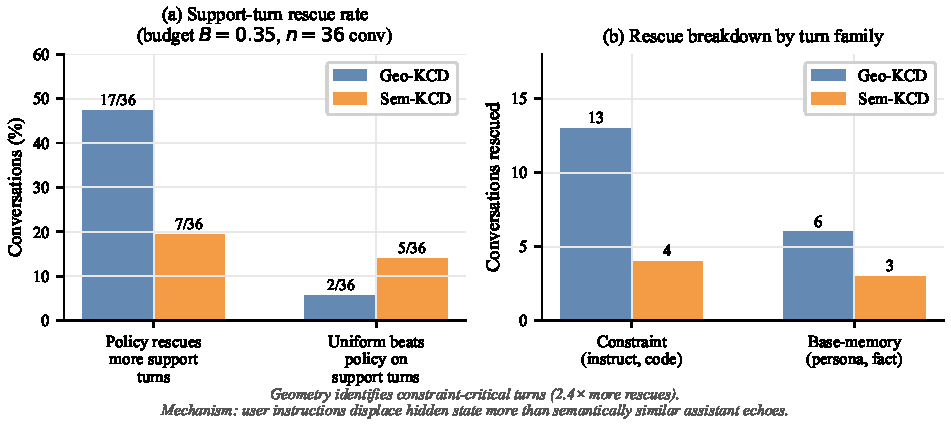
\includegraphics[width=\columnwidth]{figures/fig5_support_turn_rescue.pdf}
\caption{Support-turn rescue analysis on the hard stress set ($n{=}36$ conversations,
budget $B{=}0.35$).
\emph{Left}: overall rescue counts relative to uniform.
\emph{Right}: breakdown by turn family.
Geo-KCD rescues $2.4\times$ more constraint-critical turns than Sem-KCD.}
\label{fig:rescue}
\end{figure}

% ---------------------------------------------------------------
\section{Scope Conditions}
\label{sec:scope}
% ---------------------------------------------------------------

The results above establish the efficacy of geometry-based scoring
under specific conditions.
We now characterize two scope conditions that bound these claims.

\subsection{Architecture Dependence}

\begin{table}[t]
\centering
\caption{Cross-architecture comparison on MSC valid ($n{=}50$ conversations)
with Llama-3.2-3B-Instruct.
Lower is better. $\Delta$NLL (conv) = \semkcd{} minus \geokcd{} at conversation
level; negative means \semkcd{} is better.}
\label{tab:llama}
\setlength{\tabcolsep}{4.5pt}
\begin{tabular}{lcccccc}
\toprule
& \multicolumn{3}{c}{Logit $\ell_2$ $\downarrow$} & \multicolumn{3}{c}{Answer NLL $\downarrow$} \\
\cmidrule(lr){2-4}\cmidrule(lr){5-7}
Policy & $B{=}0.20$ & $B{=}0.35$ & $B{=}0.50$ & $B{=}0.20$ & $B{=}0.35$ & $B{=}0.50$ \\
\midrule
Uniform   & 689.7 & 669.4 & 631.0 & 3.722 & 3.657 & 3.524 \\
\geokcd{} & 690.6 & 643.2 & 592.2 & 3.617 & 3.416 & 3.260 \\
\semkcd{} & \textbf{671.9} & \textbf{633.5} & \textbf{586.1} & \textbf{3.526} & \textbf{3.317} & \textbf{3.139} \\
\midrule
$\Delta$NLL (conv) & \multicolumn{3}{c}{$-0.091^{**}$\;$-0.099^{*}$\;$-0.121^{**}$}
                   & \multicolumn{3}{c}{$p = 0.007$\;$0.026$\;$0.009$} \\
\bottomrule
\end{tabular}
\end{table}

On Llama-3.2-3B-Instruct (Table~\ref{tab:llama}),
semantic compression \emph{significantly outperforms} geometry at all budgets
for behavioral quality ($p \leq 0.026$ conversation level),
and the logit $\ell_2$ advantage of semantic is not significant at any budget
($p \geq 0.14$).
This is the opposite of the Qwen pattern.

We attribute this to pretraining regime differences.
Instruction-following finetuning via RLHF or instruction tuning
\citep{ouyang-etal-2022-training, wei-etal-2022-finetuned}
reshapes the model's representational geometry to respond more sharply
to directive content (user instructions, constraints, factual assertions).
Qwen2.5 models undergo heavy such finetuning,
producing discriminative per-turn geometry where user instructions
reliably move the hidden state more than assistant echoes.
Llama-3.2-3B's training does not produce this property to the same degree;
the geometric signature of constraint-critical turns is weaker,
making semantic similarity the more reliable selection criterion.
The scope condition is therefore about the model's representational structure
induced by its training regime, not parameter count.

\subsection{Length Dependence}

\begin{table}[t]
\centering
\caption{Cross-benchmark results on \lme{} ($n{=}100$ full-length conversations,
400--600 turns, Qwen2.5-1.5B, binding-budget variant: recent-window\,=\,0). Lower is better.}
\label{tab:lme}
\setlength{\tabcolsep}{5pt}
\begin{tabular}{lcccccc}
\toprule
& \multicolumn{3}{c}{Logit $\ell_2$ $\downarrow$} & \multicolumn{3}{c}{Answer NLL $\downarrow$} \\
\cmidrule(lr){2-4}\cmidrule(lr){5-7}
Policy & $B{=}0.20$ & $B{=}0.35$ & $B{=}0.50$ & $B{=}0.20$ & $B{=}0.35$ & $B{=}0.50$ \\
\midrule
Uniform   & 1750.7 & 1781.8 & 1714.2 & 0.222 & 0.191 & 0.141 \\
\geokcd{} & 1763.0 & 1701.3 & \textbf{1683.4} & 0.135 & 0.109 & 0.096 \\
\semkcd{} & \textbf{1750.6} & \textbf{1700.5} & 1717.9 & \textbf{0.100} & \textbf{0.096} & \textbf{0.094} \\
\semqcg{} & 1755.9 & 1748.1 & 1705.0 & 0.108 & 0.105 & 0.099 \\
\bottomrule
\end{tabular}
\end{table}

Table~\ref{tab:lme} shows results on \lme{} \citep{wu-etal-2025-longmemeval},
a benchmark of episodic retrieval tasks with 400--600 turn conversations
(no truncation).
All \kcd{} policies improve behavioral quality versus uniform
($p < 0.05$ at conversation level for all NLL comparisons at budgets $0.20$--$0.35$),
confirming that turn-level selection generalizes across benchmarks.

However, the geometry advantage does \emph{not} replicate at conversation level---
the pattern fully reverses.
At budget $0.35$, \semqcg{} is significantly \emph{worse} than \semkcd{} on
\emph{both} metrics: logit $\ell_2$ ($\Delta{=}{+}47.6$, $p_\text{conv} = 0.018$)
and answer NLL ($\Delta{=}{+}0.012$, $p_\text{conv} = 0.001$).
At budget $0.50$, the L2 difference is not significant ($p_\text{conv} = 0.629$),
but \semqcg{} remains significantly worse on NLL ($\Delta{=}{+}0.006$,
$p_\text{conv} < 0.001$; see Table~\ref{tab:lme_pairwise} in the Appendix).
\semkcd{} achieves the best NLL across all budgets
($0.100$ at $B{=}0.20$, vs.\ $0.222$ for uniform; $p<0.001$).
This reversal has a natural explanation:
in 400--600 turn conversations, each turn's geometric signature is competing
with hundreds of other turns in a crowded representational space.
Per-turn geometric features become noisier as trajectory length grows,
because individual displacement vectors represent smaller fractions of
the total trajectory variance.
Semantic shortlisting, which operates at coarser granularity,
remains discriminative; geometry provides no additional value within
a crowded shortlist.

\paragraph{Summary.}
The geometry advantage is reliable for conversations of roughly $20$--$100$ turns
(MSC regime): at budget $0.50$, \semqcg{} beats uniform on both geometry
and behavior---the only regime in our experiments where any compression policy
is strictly more faithful than no selection.
For very long conversations ($>400$ turns), the advantage inverts:
\semkcd{} dominates on both metrics and \semqcg{} underperforms it
on NLL at all budgets.
Signal design should therefore be conditioned on expected conversation length.

\begin{figure}[t]
\centering
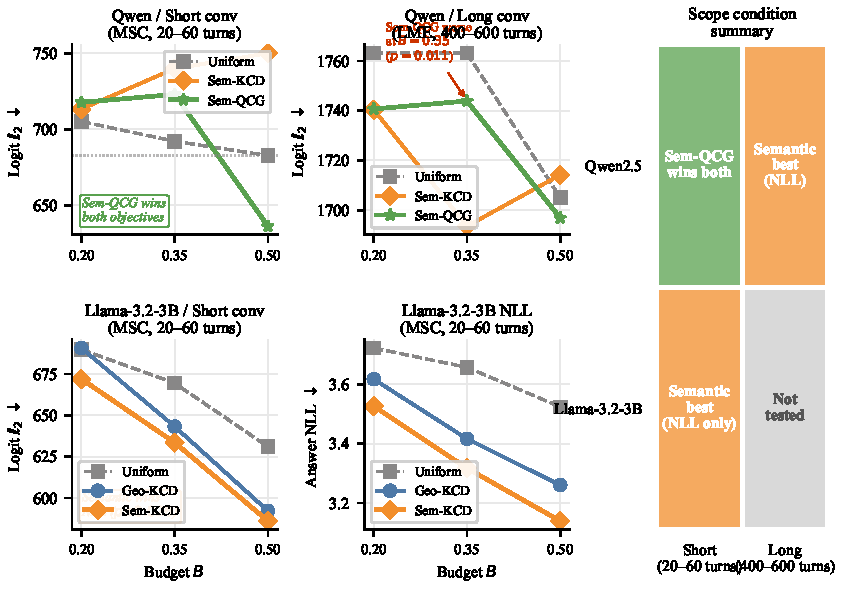
\includegraphics[width=\columnwidth]{figures/fig6_scope_conditions.pdf}
\caption{Scope condition map.
Rows: model family. Columns: conversation length regime.
\emph{Green (Sem-QCG wins both)}: query-conditioned geometry resolves the
geometry-behavior tradeoff on Qwen + short conversations.
\emph{Orange (Semantic best)}: semantic scoring dominates on Llama and on
long conversations where per-turn geometry is noisy.
Right panel summarizes the 2$\times$2 grid.}
\label{fig:scope}
\end{figure}

% ---------------------------------------------------------------
\section{Related Work}
\label{sec:related}
% ---------------------------------------------------------------

\paragraph{Prompt and context compression.}
\citet{jiang-etal-2024-longllmlingua} propose perplexity-guided
token-level compression for long-context LLM inference.
We use LongLLMLingua as a primary baseline and show it achieves
only marginal NLL improvement while incurring large geometric degradation---
evidence that NLL-optimized compression is not sufficient for representational fidelity.
\citet{pan-etal-2024-llmlingua2} propose LLMLingua-2, a data-distillation
approach for task-agnostic prompt compression.
\citet{chevalier-etal-2023-adapting} use language model fine-tuning to learn
compact memory representations; our approach operates at inference time
without modifying model weights.
\citet{he-etal-2025-pretraining} train a context compressor as a preprocessing step.

A complementary line of work compresses the KV cache at the \emph{token} level
during generation.
\citet{zhang-etal-2023-h2o} retain ``heavy hitter'' tokens---those with the
largest cumulative attention mass---discarding the rest dynamically.
\citet{li-etal-2024-snapkv} identify which prompt tokens the model will attend
to before generation begins and snap the cache accordingly.
\citet{cai-etal-2024-pyramidkv} vary the cache budget across transformer layers
in a pyramidal schedule.
\citet{nawrot-etal-2024-dynamic} learn to merge and evict KV slots during training.
All four operate at sub-token granularity within the KV cache;
our \kcd{} codec operates at turn granularity and introduces a dual geometric--behavioral
evaluation objective that none of these methods consider.

\paragraph{Conversational memory and benchmarks.}
\citet{xu-etal-2022-beyond} introduce Multi-Session Conversations (MSC),
a persona-grounded multi-session dialogue dataset that we use as
our primary evaluation benchmark.
\citet{wu-etal-2025-longmemeval} introduce LongMemEval,
testing five core memory abilities across 500 manually curated questions
embedded in scalable user-assistant chat histories.
\citet{maharana-etal-2024-evaluating} develop LoCoMo,
a benchmark for very-long-term conversational memory.
\citet{luo-etal-2026-from} survey memory mechanisms in LLM agents,
classifying them into context-resident compression, retrieval-augmented stores,
reflective self-improvement, hierarchical virtual context, and policy-learned management;
our \kcd{} codec falls in the context-resident compression family.
\citet{nan-etal-2025-nemori} propose Nemori, a self-organizing memory system
inspired by cognitive science.
\citet{wang-etal-2025-hymem} introduce HyMem, a hybrid memory architecture
with dynamic retrieval scheduling.

\paragraph{Retrieval and external memory.}
An orthogonal strategy is to externalise history into a retrieval index.
\citet{lewis-etal-2020-retrieval} introduce retrieval-augmented generation (RAG),
which retrieves relevant documents at query time rather than compressing
the context window.
\citet{packer-etal-2023-memgpt} treat the LLM context window as a fast memory
tier and implement page-in/page-out semantics to a slower external store.
Our approach is complementary: we compress within the context window at
inference time without an external index or modified architecture,
and we measure the geometric cost of compression decisions---a cost that
retrieval-based systems incur implicitly when summarising or dropping history.

\paragraph{Hidden-state geometry in language models.}
Transformer representations are known to occupy a compact, anisotropic subspace.
\citet{ethayarajh-2019-contextual} show that contextualized embeddings are far
from isotropic: upper-layer representations are highly context-specific,
with less than $5\%$ of variance explained by static word identity.
\citet{cai-etal-2021-isotropy} further characterize the cluster structure of
this embedding space and introduce a rigorous isotropy measure.
These findings motivate our Rank-95 metric, which quantifies how compactly
conversation trajectories occupy $\mathbb{S}^{d-1}$;
the theoretical basis for such dimensionality measures is established in
\citet{li-etal-2018-measuring} and \citet{aghajanyan-etal-2021-intrinsic}.
\citet{huh-etal-2024-platonic} observe cross-model convergence of representations
toward a shared geometric structure, motivating our cross-architecture comparisons.
\citet{xiao-etal-2023-efficient} identify attention sinks---tokens that
accumulate disproportionate attention mass---which we correct for in
hidden-state extraction.
\citet{anagnostidis-etal-2022-signal} provide theoretical grounding
for the low Rank-95 values we observe ($1.05$--$1.53$).
To our knowledge, we are the first to use \emph{parallel-transported geometry}
on conversation-state trajectories as a turn-selection signal.

% ---------------------------------------------------------------
\section{Geometry Characterization}
\label{sec:geomchar}
% ---------------------------------------------------------------

We present supporting evidence for our geometric motivation.

\begin{table}[t]
\centering
\caption{Geometry characterization across model families.
Rank-95: intrinsic dimensionality of conversation trajectories
(lower = more compact, normalized by trajectory length).
Shuffled Rank-95: control with turn order randomized.
$\rho$: Pearson correlation between per-turn geometric distortion and
logit $\ell_2$ (H3: geometry predicts decoder drift).
All $p$ values from conversation-level permutation tests.}
\label{tab:geometry}
\begin{tabular}{lccccc}
\toprule
Model & Rank-95 & Shuffled & $p_{H_1}$ & $\rho$ & $p_{H_3}$ \\
\midrule
Qwen2.5-0.5B & $1.049$ & $1.486$ & $<0.001$ & $0.989$ & $<0.001$ \\
Qwen2.5-1.5B & $1.167$ & $1.458$ & $0.001$  & $0.994$ & $<0.001$ \\
SmolLM2-1.7B & $1.528$ & $1.799$ & $0.012$  & $0.989$ & $<0.001$ \\
\bottomrule
\end{tabular}
\end{table}

Table~\ref{tab:geometry} shows that:
(H1) Real conversation trajectories are significantly more compact than shuffled
controls ($p \leq 0.012$), confirming temporal ordering creates compact geometry.
(H3) Per-turn geometric distortion tightly predicts decoder drift
($\rho = 0.989$--$0.994$, $p < 0.001$), confirming geometric distortion
is a meaningful proxy for representational harm.
These properties hold across architectures and parameter scales.

\begin{figure}[t]
\centering
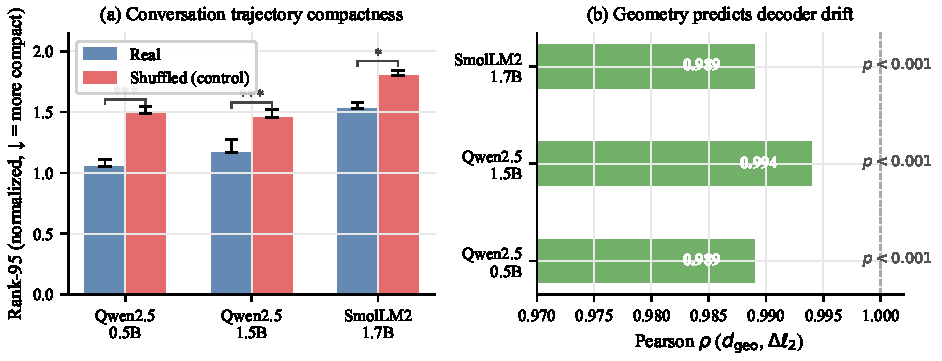
\includegraphics[width=\columnwidth]{figures/fig2_geometry_characterization.pdf}
\caption{Geometry characterization across model families.
\emph{Left}: Rank-95 for real vs.\ shuffled conversation trajectories.
Real trajectories are significantly more compact ($p \leq 0.012$).
\emph{Right}: Pearson $\rho$ between per-turn geometric distortion and
logit $\ell_2$ ($\rho = 0.989$--$0.994$, all $p{<}0.001$).}
\label{fig:geomchar}
\end{figure}


% ---------------------------------------------------------------
\section{Limitations}
\label{sec:limits}
% ---------------------------------------------------------------

\paragraph{Architecture dependence.}
The geometry advantage is not universal.
On Llama-3.2-3B-Instruct, semantic compression significantly outperforms
geometry-based compression for behavioral quality ($p \leq 0.026$, all budgets).
We attribute this to pretraining differences,
but do not test this hypothesis directly.
Practitioners should validate geometric scoring on their target model family
before deployment, using a held-out development set.

\paragraph{Conversation length dependence.}
The geometry advantage degrades on 400--600 turn conversations
(\lme{} benchmark):
\semqcg{} is significantly \emph{worse} than \semkcd{} on logit $\ell_2$
at $B{=}0.35$ ($p_\text{conv} = 0.011$).
Per-turn geometric features become less discriminative as trajectory length grows.
Our MSC experiments use conversations of 20--60 turns;
results may not generalize to much longer sessions without adaptation.

\paragraph{Oracle metric circularity.}
Our support-turn rescue analysis identifies support turns by manual annotation
on a small synthetic stress set ($36$ conversations).
This is a qualitative mechanism study, not a large-scale validation.
The claim that geometry detects constraint-critical turns rests on
this small-$n$ analysis plus the signal-swap effect sizes in Table~\ref{tab:hardset}.

\paragraph{QA evaluation on LME.}
We ran a QA proxy evaluation on LME using the next conversation turn
as the gold answer.
Token F1 scores were uniformly near-zero ($\approx 0.08$) across all policies,
and we determined this metric is invalid because
LME's conversational gold turns are not faithful proxies for the
question-answer pairs in the official evaluation protocol.
We therefore do not report these results as primary evidence
and rely on NLL and logit $\ell_2$ for the LME cross-benchmark analysis.

\paragraph{Scale.}
Our experiments use models up to 3B parameters.
We do not test 7B+ models due to compute constraints.
The observed scale trend (NLL damage grows 1.5B $\to$ 3B) suggests
geometry may matter more at larger scale,
but this hypothesis requires direct validation.

% ---------------------------------------------------------------
\section{Conclusion}
% ---------------------------------------------------------------

We introduced the \kcd{} codec for conversational memory compression
and showed that the choice of turn scoring signal is a first-class
design decision.
Geometry and behavioral quality are distinct objectives that diverge
in practice:
\textsc{LongLLMLingua}, a state-of-the-art prompt compression method,
trades geometric fidelity for marginal NLL improvement.
Query-conditioned geometry inside a semantic shortlist (\semqcg{})
resolves this tradeoff on Multi-Session Conversations:
it achieves lower logit $\ell_2$ than uniform random sampling while
simultaneously improving answer NLL,
the only policy in our study to win on both objectives simultaneously.
On constraint-critical memory, geometry-based scoring substantially
outperforms semantic scoring,
with the NLL damage from the wrong signal growing from $0.63$ to $1.13$ nats
as model scale increases from 1.5B to 3B.
We characterize architecture and length as scope conditions,
and provide mechanism evidence through support-turn rescue analysis.
We hope these findings motivate dual-objective evaluation and
signal-conditioned design as standard practices in conversational memory research.

% ---------------------------------------------------------------
% BIBLIOGRAPHY
% ---------------------------------------------------------------
\bibliographystyle{acl_natbib}
\bibliography{kcd_arxiv}

% ---------------------------------------------------------------
\appendix
% ---------------------------------------------------------------

\section{Experimental Details}
\label{app:details}

\subsection{Models and Hardware}
All experiments run on Qwen2.5-1.5B-Instruct, Qwen2.5-3B-Instruct
\citep{qwen2025qwen25technicalreport},
and Llama-3.2-3B-Instruct \citep{grattafiori-etal-2024-llama3}.
Models are loaded in \texttt{bfloat16} with Flash Attention 2
\citep{dao-etal-2022-flashattention}
on NVIDIA L40S GPUs ($46$~GB VRAM).
All MSC experiments run with 7 GPUs and 2 workers per GPU
to saturate VRAM ($\approx 22$~GB per worker).

\subsection{Dataset Details}
\textbf{MSC valid}: Multi-Session Conversations validation split \citep{xu-etal-2022-beyond}.
Conversations average 5 sessions of 4--6 turns each.
All 1{,}000 conversations used for baseline comparison;
50 conversations for signal variant study (random sample, fixed seed 42).

\textbf{LongMemEval-S}: \citet{wu-etal-2025-longmemeval} benchmark.
100 full-length conversations, 400--600 turns each.
No truncation applied (evaluating compression policies, not context window limits).

\textbf{Hard stress set}: 9 synthetic conversations across three families
(long-dependency, retrieval-heavy, code-conversation),
$540$ evaluation rows, hand-constructed by the authors
to maximize signal-to-noise difficulty for support-turn detection.

\subsection{Compression Parameters}
Budget fractions: $B \in \{0.20, 0.35, 0.50\}$.
KCD compression ratio: $\alpha = 0.5$ (compressed turns retain half their tokens,
selected by leading-token truncation).
Semantic shortlist size for \semqcg{}: top-$k$ turns where
$k = \lceil 2B \cdot T \rceil$ (twice the keep budget, so geometry
selects the final $B \cdot T$ from $2B \cdot T$ candidates).

\subsection{Statistical Protocol}
All significance tests are two-sided signflip permutation tests
with 5{,}000 resampling iterations.
We report both row-level (anti-conservative) and conversation-level
(conservative, primary) $p$-values.
No multiple-comparison correction is applied within individual tables;
results are interpreted directionally, and effect sizes are reported
alongside $p$-values.

\subsection{Geometry Feature Extraction}
Hidden states are extracted from the final transformer layer,
normalized to the unit sphere.
Parallel transport uses the exponential and logarithm maps on $\mathbb{S}^{d-1}$:
\[
\Log_{\mathbf{p}}(\mathbf{q}) = \frac{\arccos(\mathbf{p}^\top \mathbf{q})}{\sqrt{1 - (\mathbf{p}^\top \mathbf{q})^2}}(\mathbf{q} - (\mathbf{p}^\top \mathbf{q})\mathbf{p})
\]
Reference point $\hv_\text{ref}$ is the Fréchet mean of the trajectory,
approximated by iterative geodesic midpoints.
Attention weights (for the attention-augmented feature set) are averaged
over the final 4 transformer layers with sink correction:
the first 32 tokens are excluded from weight normalization
following \citet{xiao-etal-2023-efficient}.

\section{Additional Pairwise Results}
\label{app:pairwise}

\subsection{LME Pairwise: \semqcg{} vs.\ \semkcd{}}
\begin{table}[h]
\centering
\caption{\semqcg{} minus \semkcd{} on \lme{} ($n{=}100$ conversations).
Positive $\Delta$ logit L2 means \semqcg{} is geometrically \emph{worse}.}
\label{tab:lme_pairwise}
\setlength{\tabcolsep}{4pt}
\begin{tabular}{lcccccc}
\toprule
Budget & $\Delta$ L2 (row) & $p_\text{row}$ & $\Delta$ L2 (conv) & $p_\text{conv}$ & $\Delta$ NLL (conv) & $p_\text{conv}$ \\
\midrule
$0.20$ & $+5.2$  & $0.476$ & $+5.2$  & $0.742$ & $+0.010$ & $0.738$ \\
$0.35$ & $+47.6$ & ${<}0.001$ & $+47.6$ & $0.018$ & $+0.012$ & $0.001$ \\
$0.50$ & $-12.9$ & $0.108$ & $-12.9$ & $0.629$ & $+0.006$ & ${<}0.001$ \\
\bottomrule
\end{tabular}
\end{table}

\subsection{Llama-3.2-3B Pairwise: \semkcd{} vs.\ \geokcd{}}
\begin{table}[h]
\centering
\caption{\semkcd{} minus \geokcd{} on Llama-3.2-3B ($n{=}50$ conversations).
Negative $\Delta$ NLL means \semkcd{} is better behaviorally.}
\label{tab:llama_pairwise}
\setlength{\tabcolsep}{4pt}
\begin{tabular}{lcccc}
\toprule
Budget & $\Delta$ L2 (conv) & $p_\text{conv}$ & $\Delta$ NLL (conv) & $p_\text{conv}$ \\
\midrule
$0.20$ & $-18.7$ & $0.141$ & $-0.091$ & $\mathbf{0.007}$ \\
$0.35$ & $-9.7$  & $0.514$ & $-0.099$ & $\mathbf{0.026}$ \\
$0.50$ & $-6.1$  & $0.778$ & $-0.121$ & $\mathbf{0.009}$ \\
\bottomrule
\end{tabular}
\end{table}

\end{document}
